% BlockChain %
A BlockChain or \textbf{\q{The Truth Machine}} ~\cite{the_truth_machine} can be broadly described as a peer-to-peer network of nodes that makes a collaborative effort in sensing certain specified chain of blocks of data around its periphery and thereby controls the surrounding environment.
Accrrding to Wikipedia~\cite{blockchain_wiki} a blockchain, originally block-chain, is a growing list of records, called blocks, which are linked using cryptography. Each block contains a cryptographic hash of the previous block, a timestamp, and transaction data (generally represented as a Merkle tree).
In BlockChains, each node consists of processing capability, it may contain multiple types of memory like program, data and memories, having a Web-Service transceiver, Client-side processors, and a power source. The nodes communicate with each other using web-services and self-organized.
There are certain nodes called miners that veryfies each transactions or entry of data in the chain and are the most reliable personnel in the network who always have the updated copy of blocks of data.

\begin{figure}
\begin{center}
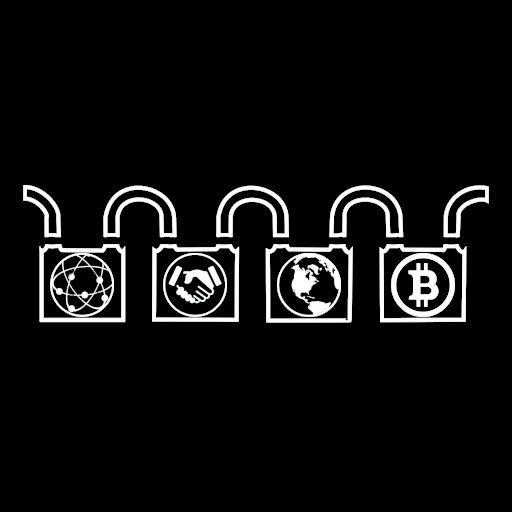
\includegraphics[width=0.5\textwidth]{./img_src/blockchain.jpg}
\end{center}
\caption{Overview of Block-Chain Technology (BCTs).}
\end{figure}

\subsection{What is Blockchain}
By definition blockchain is a decentralized computation and information sharing platform which enables multiple authoritative domains who do not trust each other to cooperate coordinate and collaborate in a rational decision making process.

The technology is particularly useful when multiple parties or individual they want to cooperate it with each other, and they want to come to a common platform to share the information among themselves.

Blockchain is that whenever we are talking about multiple authoritative domains.

This multiple authoritative domains they do not trust each other. So, this is an important aspect of blockchain that you can combine multiple authoritative domains who do not trust with each other and they can come to a common platform where they can cooperate, coordinate and collaborate in application development process at the business intelligence process.

Let's suppose in a blockchain platform Alice has her own copy of a document and Bob has his own copy of another document. So, the seperate copy belongs to Alice and Bob, and they can simultaneously write to their own document and here I have the network in between and the network has the task to ensure that the information consistencies maintained between the documents which Bob and Alice hold individually.

The advantage  is that that they do not need to rely on the internet or if a server crashes they do not depend on the server files.

So, by definition we can say that a blockchain is decentralized data based platform with strong consistency support.

\subsection{Blockchain Arcitecture}
So, the protocol for commitment means whenever someone is making a new transaction, during that time you need to ensure that this particular transaction if it is valid, it will get committed to the existing public ledger or the existing blockchain, otherwise that entry will not be there in the blockchain. So, there should be a mechanism for validity checking of every upcoming transactions from the clients and then based on that validity checking you will be able to either accept the transaction and include it in the existing blockchain or you can delete the transaction or discard the transaction.

The second requirements is a consensus. Consensus is an important aspect in the in the context of blockchain. So, in case of blockchain as we have discussed that everyone has a 
local copy of the information available to every individual parties and there is no such central platform like a bank which will maintain the consistency of the transactions or 
the consistency of the information. So, that is why the consensus mechanism ensures that whatever local copy every individual party has they are consistent with each other that 
everyone has the most updated copy, and a copy, that the individuals have, are identical or similar to each other. 

The third important aspect is the security. That means, the data that one is inserting in a public ledger or inside the blockchain, now because this blockchain is distributed to individual parties everyone is maintaining their local copy of the blockchain. So, that person may change something in that local copy and broadcast that saying that \q{see this is the updated information}.

Fourth aspects is the privacy and authenticity. The data or the transactions which is their inside the blockchain it belong to various clients. So, it is coming from various clients and you are putting that information inside the blockchain and a copy of the blockchain is available to every parties and that is why the privacy and authenticity of the information needs to be ensured.

Some of the underlying concepts of the BlockChain especially BitCoin (the most popular implementation of BlockChain) and some other important technology are briefed.

\subsection{Types}
There are two types of blockchain,

\subsubsection{Permissionless BlockChain}
Permissionless or Public blockchain networks power up most of the market's digital currencies. They allow every user to create a personal address and begin interacting with the network, by submitting transactions, and hence adding entries to the ledger. Additionally, all parties have the choice of running a node on the system, or employing the mining protocols to help verify transactions.

Additionally, for digital currencies such as Ethereum, the blockchain network also supports smart contracts, which are automated transactions that self-execute when certain criteria are met. As Ethereum also employs a permisionless blockchain, anyone can develop and add smart contracts onto the network, with no limitation imposed by the developers. Apart from allowing anyone to get involved on the network, there are few more characteristics associated with the permisionless model. These are:

\begin{itemize}
\item \textbf{Decentralization:} No central entity has the authority to edit the ledger, shut down the network, or change its protocols.
\item \textbf{Digital assets:} The presence of a financial system on the network.
\item \textbf{Anonymity:} It do not require users to submit personal information prior to being able to create an address, or submit transactions. However, in certain cases, personal information is required for legal purposes
\item \textbf{Transparency:} It needs to freely give users access to all information apart from the private keys from addresses, to how transactions are processed into blocks, and the freedom to see all transactions processed by the network.
\end{itemize}

\subsubsection{Permissioned BlockChain}
Permissioned or Private blockchain closed ecosystems, where users are not freely able to join the network, see the recorded history, or issue transactions of their own. Permissioned blockchains are preferred by centralized organizations, which leverage the power of the network for their own, internal business operations. Company consortiums are also likely to employ private blockchains to securely record transactions, and exchange information between one another.

\subsection{Peer-to-Peer Network}
This is the internet protocol that connects different logged in users as a node which is having some computation power. The users who are only uploading and verifying may have computer or smartphone, but the verifiers or the miners must have to work on computer with sufficient amount of computation power.

\begin{tikzpicture}[]
\node(node1)[node] {node1};
\node (pl1) [pl, left of=node1, xshift=-0.1cm] {};
\node(node2)[node, right of=node1, xshift=5cm] {node2};
\node (pl2) [pl, right of=node2, xshift=0.1cm] {};
\node(node3)[node, below of=node1, yshift=-3cm] {node3};
\node (pl3) [pl, left of=node3, xshift=-0.1cm] {};
\node(node4)[node, below of=node2, yshift=-3cm] {node4};
\node (pl4) [pl, right of=node4, xshift=0.1cm] {};
\node(node5)[node, right of=node1, xshift=2cm,yshift=2cm] {node5};
\node (pl5) [pl, above of=node5, yshift=0.3cm] {};
\node(node6)[node, right of=node3, xshift=2cm,yshift=-2cm] {node6};
\node (pl6) [pl, below of=node6, yshift=-0.3cm] {};

\draw[<->, thick] (node1) -- (node2);
\draw[<->, thick] (node1) -- (node3);
\draw[<->, thick] (node1) -- (node4);
\draw[<->, thick] (node1) -- (node5);
\draw[<->, thick] (node1) -- (node6);
\draw[<->, thick] (node2) -- (node3);
\draw[<->, thick] (node2) -- (node4);
\draw[<->, thick] (node2) -- (node5);
\draw[<->, thick] (node2) -- (node6);
\draw[<->, thick] (node3) -- (node4);
\draw[<->, thick] (node3) -- (node5);
\draw[<->, thick] (node3) -- (node6);
\draw[<->, thick] (node4) -- (node5);
\draw[<->, thick] (node4) -- (node6);
\draw[<->, thick] (node5) -- (node6);
\end{tikzpicture}


\subsection{Transactions}
Everything in crypto-currency comes under transactions, i.e. someone is sending some amount of money to someone else at some time. So a basic or overall transaction data can be structured as,

\fbox{\colorbox{lightgray}{\parbox[b][4cm][c]{0.50\linewidth}{
\textbf{\texttt{\noindent Transaction :: \{\\
\hspace*{1cm} \textless Transaction\_id\textgreater,\\
\hspace*{1cm} \textless TimeStamp\textgreater,\\
\hspace*{1cm} \textless Sender\_Id\textgreater,\\
\hspace*{1cm} \textless Receiver\_Id\textgreater,\\
\hspace*{1cm} \textless Amount\_Unit\textgreater\\
\noindent \}}}
}}}

This transaction details is send to every peer to verify. If they heard already about it, it is true, or it is false (same as women's un-manipulated gossip in village). If more than 50\% population declare it true, then it is allowed to be in the Public Ledger.

\subsection{Public Ledger}
This is the publicly shared record of transactions kept as a list of blocks. At a particular point of time everybody (every node), who are connected to the network, should have a same copy of ledger in their own devices of what server has. Whenever a new person logs into the network aotomatically the server forces to update the ledger to the person's device. So basically the ledger is the chain file.

\subsection{Chain of Blocks}
It means list of blocks of data having some common part with previous and next block. This is like Single-way linked-list(every node consists of data and program memory address to the next node). Every block contains a number of transactions and many more things.

\fbox{\colorbox{lightgray}{\parbox[b][6cm][c]{0.75\linewidth}{
\textbf{\texttt{\noindent Block :: \{\\
\hspace*{1cm} \textless Block\_Id\textgreater,\\
\hspace*{1cm} \textless TimeStamp\textgreater,\\
\hspace*{1cm} \textless Merkle\_Root\textgreater,\\
\hspace*{1cm} \textless Verifier\_Id\textgreater,\\
\hspace*{1cm} \textless Nonce\_Value\textgreater,\\
\hspace*{1cm} \textless Previous\_Hash\textgreater,\\
\hspace*{1cm} \textless Current\_Hash\textgreater,\\
\hspace*{1cm} \textless Data :: ANumberOfTransactions\textgreater\\
\noindent \}}}
}}}

So it is kind of backword linked-list which is propagating by having the previous block's kind of identity (because there is a mild chance of collision i.e. multiple values' hashes are same) hash.

\subsection{Timestamp}
The time means absolute global date-time in the format: 

\fbox{\colorbox{lightgray}{\parbox[b][2cm][c]{\linewidth}{
\textbf{\texttt{\noindent TimeStamp :: String (
\textless day\_of\_week\_code :: ddd\textgreater,
\textless month\_code :: mmm\textgreater,
\textless day\_of\_month :: dd\textgreater,
\textless year :: yyyy\textgreater,
\textless time :: hh:mm:ss\textgreater,
\textless Distance from Mean-TimeLine :: GMT+hhmm\textgreater,
\textless Time Zone :: Country\_Name Standard Time\textgreater
\noindent )}}
}}}

Example: \textbf{\q{Sat May 25 2019 20:45:04 GMT+0530 (India Standard Time)}}. The timestamp is one of the most needed to prove it later for verification of the record. It is used to create the current block's hash.

\subsection{Hash}
The job of a hash algorithm is to map any size of domain to a particular size of range. SHA-256 is one of the most popular hash algorithms which takes any length input and returns 256 bit output. All input/output operations can be transferred into strings.

\subsection{Merkle Root Hash}
Merkle tree is a complete binary tree which has the hash values of transaction data as leaf nodes. The tree propagation occures from leaves to root as tournament tree form. For any point,

			parent hash = hash(child-1 hash + child-2 hash);

A little change in any data of any transaction will change the merkle root, and thus the block's hash and the complete chain. Because it is used to create the current block's hash.

\begin{tikzpicture}[]
\node (root) [process] {H\_r = hash(H\_0 + H\_1)};
\node (child1) [process, below of=root, xshift=-4cm, yshift=-2cm]{H\_0 = hash(H\_0-0 + H\_0-1)};
\node (child2) [process, below of=root, xshift=4cm, yshift=-2cm]{H\_1 = hash(H\_1-0 + H\_1-1)};
\node (child3) [process, below of=child1, xshift=-2cm, yshift=-2cm]{hash(TxD\_0)};
\node (child4) [process, below of=child1, xshift=2cm, yshift=-2cm]{hash(TxD\_1)};
\node (child5) [process, below of=child2, xshift=-2cm, yshift=-2cm]{hash(TxD\_2)};
\node (child6) [process, below of=child2, xshift=2cm, yshift=-2cm]{hash(TxD\_3)};

\node (txd0) [process, below of=child3, yshift=-2cm] {TxD\_0};
\node (txd1) [process, below of=child4, yshift=-2cm] {TxD\_1};
\node (txd2) [process, below of=child5, yshift=-2cm] {TxD\_2};
\node (txd3) [process, below of=child6, yshift=-2cm] {TxD\_3};

\draw [arrow] (child1) -- (root);
\draw [arrow] (child2) -- (root);
\draw [arrow] (child3) -- (child1);
\draw [arrow] (child4) -- (child1);
\draw [arrow] (child5) -- (child2);
\draw [arrow] (child6) -- (child2);
\end{tikzpicture}


\subsection{Previous Hash}
The previous block's hash. It is required to maintain the chain system because we can not create the next address and we don't know when it would be created, so it is better to store what we already have. It is used to create the current block's hash.

\subsection{Nonce}
It is the quantity of computation power used to solve a mathematical problem which is not so hard but not so easy either. Too easy solution will be easy to break and too hard solution will take so long time to create a block that the adversary with huge computation power have a chance to alter the data before creating and verifying a block. Rather a medium hard problem will be better. It is used to create the current block's hash.

This is to show the verifiers that the block creator have spent sufficient amount of computation power before creating the block and also to delay the process a little bit and this is called POW (Proof of Work). In bitcoin the problem is to find the first hash of given values which is having 'd' number of leading 'zero's where the 'd' represents the difficulty of the problem i.e. the more 'd' gets it will take longer to calculate. Typical value of 'd' is 32 bits and average delay for the whole block addition (create, verify then add) is about 10 minutes.

\subsection{Consensus Mechanism}
It is the contract or the protocol by which the blocks are verified and the winning blocks are added to everyone's ledger as well as the central server. The actual consensus algorithm is not published for security reasons. But by possible ways or reverse eengineering people have created  different models. Some of those models are:

\begin{figure}
\begin{center}
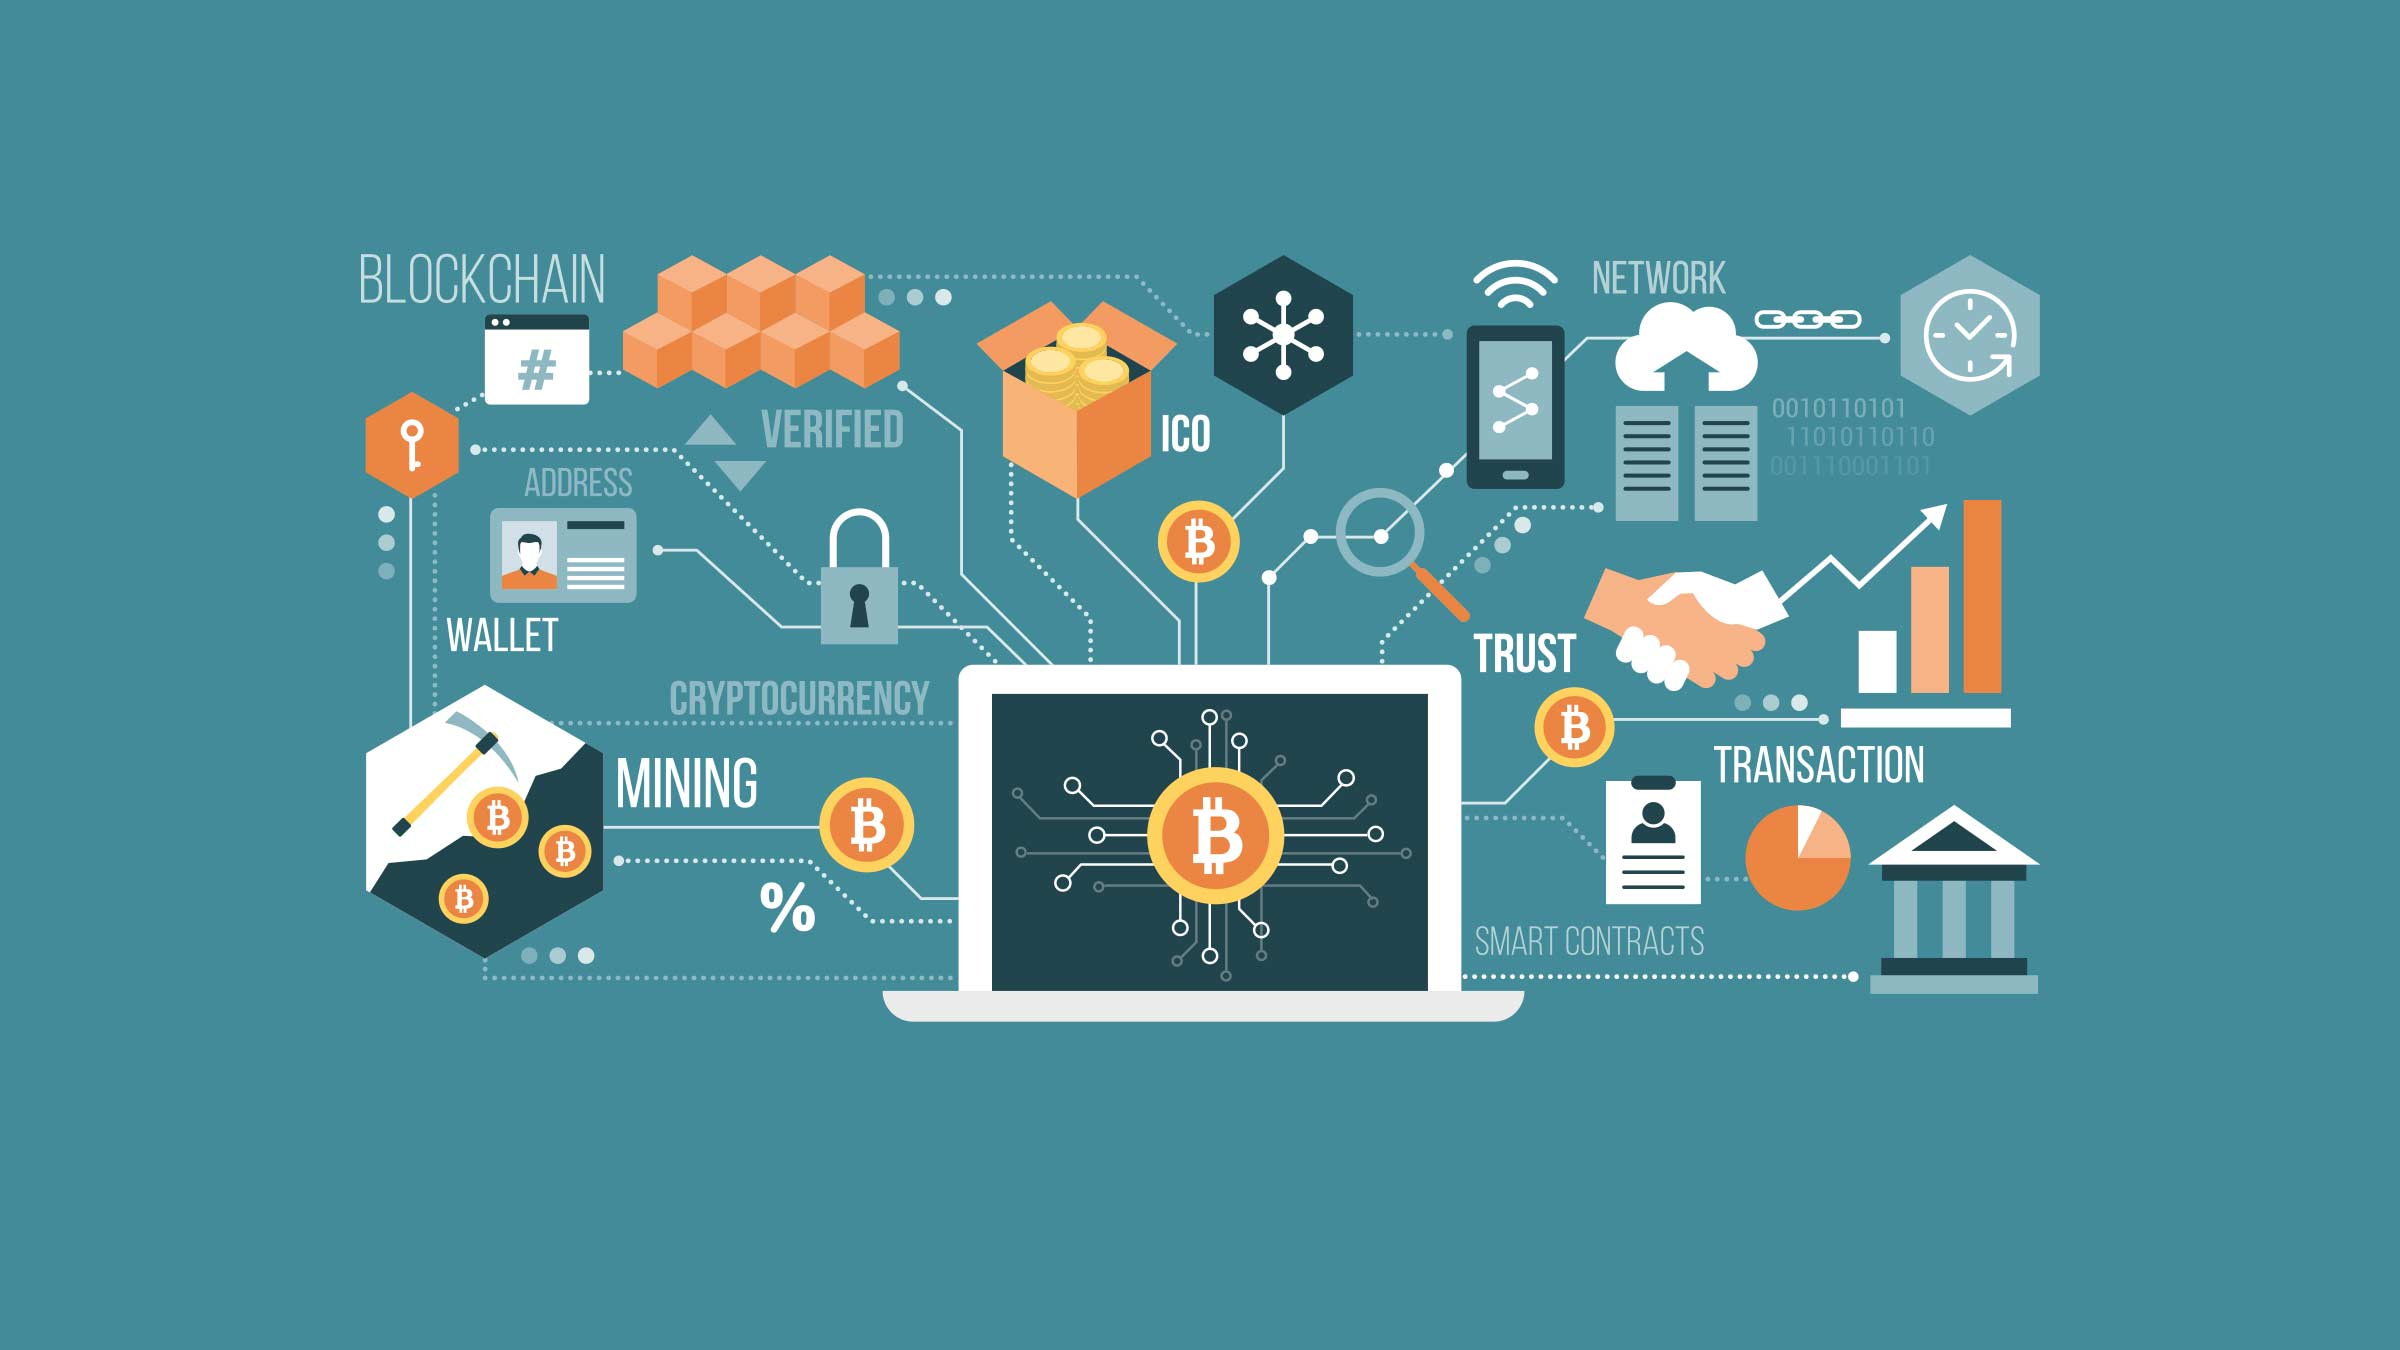
\includegraphics[width=0.75\textwidth]{./img_src/bitcoin.jpg}
\end{center}
\caption{Overview of BitCoin Technology (BCTs).}
\end{figure}

\begin{enumerate}
\item Probable bitcoin consensus mechanism
\item Paxos (Part-Time Parliament) consensus mechanism~\cite{paxos_made_easy, paxos_made_practical}
\item Raft consensus mechanism~\cite{raft_extd}
\end{enumerate}

Bitcoins one is probably the simplest one, but having bugs. The Paxos allows different types of sources and faults to come, it learns and fixes it. Raft does not allow any fault to happen.

The basic overall way in which consensus happen in bitcoin might be the following,

\begin{enumerate}
\item The transaction comes to server from client nodes;
\item Server stores that in file system database as unverified transaction;
\item At the point of interval of 10 minutes server broadcasts it to the miners network i.e. to every miner;
\item Each miner individually verifies and adds correct transaction in a block. Each node holds its block creation and validates the new block as soon as it gets new block from network. Who's block is valid and introduced first to network will be added to everyone's chain and they will start making new block on top of it. Sometimes forks might be created for the networking distance between distant nodes, at that moment conflict will come. If a new introduced block's previous hash does not match with the last block's current hash the node requests to the network to get the missing blocks one by one until the blocks match, it validates it, delete the wrong blocks (make them orphan) and add missing blocks to own chain to resolve fork and maintain longest updated chain. So it is a race between miner nodes.
\item Server gets a copy from miners group and updates own copy and delete the added tansactions from file system.
\end{enumerate}

\subsection{Applications of BCTs}
Block-Chain Technology provides one major advantage over conventional centralized database system: immunity from unexpected data changes or Hacks, which gives rise to numerous applications. Some of them include

\begin{itemize}
\item Crypto-currency: Creating and transferring digital money, Data Mining.
\item Military applications: Secure and verified records of Every Military Events and documents.
\item Structural health Monitoring
\item e-Biding Systems
\item Election System or e-Voting Systems
\item Selling Records and other Commercial Applications
\item Music Copyright Verification System
\item Integrity Analysis of Media Files
\end{itemize}

\subsection{Application}
Some of the commercial applications built on blockchain technology are as follows,

\subsubsection{BitCoin}
One year after creating protocols of BlockChian for cryptocurrency, Satoshi Nakamoto in 2009 released the first source code for BitCoin (BTC) application. Bitcoin has since grown rapidly to a market footprint of around 39 billion U.S. dollars (as of 12 Jul 2017). BTC is a decentralized cryptocurrency using a permissionless blockchain that every user has the ability to download and thereby check. The users of the network use their personal computational power to verify transactions through hashes, i.e., mining. The total computational power of the Bitcoin network is estimated to be more than 256 times the power of the world's 500 top supercomputers.
Site: \href{https://bitcoin.org/}{BitCoin}.

\subsubsection{HyperLedger}
Hyperledger is a project under the Linux Foundation which seeks to provide a unified blockchain architecture for industrial applications. Hyperledger is a collaboration of more than 100 organizations focused on banking, supply chain, and other transaction networks. It uses BFT system to reach consensus by fewer number of nodes.
\href{https://www.hyperledger.org/}{HyperLedger}

\subsubsection{Ethereum}
It is a permissionless blockchain made as a smart contracts platform run by Ether (ETH). The verification is done through the peer to peer network which constitutes Ethereum together with ETH which fuels the network, the consensus algorithm to share the state of the network, and the Turing complete scripting language which enables users to write complex scripts (smart contracts). It is the consensus engine which sets the speed of the Ethereum network by updating the state of the network at specific time intervals (shorter than for the Bitcoin network). The Ethereum network is fueled by gas which is a unit connected to ETH which is used to pay for the storage and computations an application (smart contract) needs.
\href{https://www.ethereum.org/}{Ethereum}

Solidity is a programing language build specifically to target the Ethereum virtual Machine (EVM) which in turn is the protocol to access the blockchain. Solidity has a syntax similar to JavaScript and is the language in which many smart contracts are written. The smart contracts are then compiled into bytecode and fed into to EVM and thus they can operate on the blockchain. In Ethereum are every transaction and smart contract is saved on the blockchain. The blockchain is in turn distributed and the states are handled by the consensus algorithm.
\href{https://solidity.readthedocs.io/en/v0.5.7/}{Solidity}

\subsubsection{Tendermint}
Tendermint is not a blockchain in itself but rather a general purpose blockchain consensus engine with a consensus layer for blockchaining. Tendermint can be used as a replacement for the consensus engines of other blockchains. It runs BFT algorithm.
\href{https://tendermint.com/}{Tendermint}

\subsubsection{Eris:db}
Eris:db is a controllable (permissible), smart contract-enabled, PoS based blockchain design with the PoS based on Tendermint. Eris:db is an application layer for blockchain applications. Eris is the backbone for deploying and interacting with the application logic.
\href{https://github.com/vulcanize/eris-db}{Eris:db}

\subsubsection{Cumulus}
Cumulus is a blockchain solution developed by Ericsson. Cumulus builds on and works with the Ethereum Virtual Machine (EVM) but separates the consensus algorithm and the blockchain from the EVM. Cumulus works similar to Ethereum; however, it is a private blockchain which means it does not run on gas.
\href{https://github.com/ubclaunchpad/cumulus}{Cumulus}

\subsection{Comparison}
There are a number of blockchain solutions to choose from, some of the most important ones are described in the previous subsections. For this thesis we will use a hybrid one, that supplies our requirements or logical proposal.

\begin{center}
\begin{tabular}{|c|c|c|c|c|c|}
\hline
\textbf{Name} & \textbf{Distribution} & \textbf{Transactions/second} & \textbf{Consensus Algorithm} \\
\hline
\textbf{Hyperledger} & Private & 10k & BFT \\
\hline
\textbf{Eris:db} & Private & 10k & Tendermint(PoS) \\
\hline
\textbf{Ethereum} & Public & 20 & PoS \\
\hline
\textbf{Tendermint} & Private & 10k & Tendermint BFT \\
\hline
\textbf{Bitcoin} & Public & 7 & PoW \\
\hline
\textbf{Cumulus} & Private & (untested) & (unknown) \\
\hline
\end{tabular}
\end{center}

\subsection{Security and Integrity in BCTs}
As the data is not sitting on a single data server so there is no security issue for Server Hacking. And also the hash-Chain with Cryptography makes it near to impossible to figure out or change previous data block in the blockchain. Before adding any data block with the help of consensus mechanism the blocks are verified with the digital signature of the node and some solution of nonce (the number of times the cllient application required to calculate the mathematical problem) and various other meta data.
As in some interval the system is refreshing itself, if some error seems to be occured, it backs up itself by contacting the miners (the trusted nodes), compare their files and back up with the valid one. So no integrity problem is there, unless and until the internet works fine.
